% !TEX program = xelatex
% DINOv2 arXiv 2304.07193v2 / TMLR 01/2024, Sections 3-7, Appendix A-B.
% Original imagegen draft retained unchanged via graphicx viewports.
% All math, Chinese labels, arrows and grouping redrawn precisely in TikZ.
\documentclass[tikz,border=2mm]{standalone}
\usepackage{fontspec,xeCJK,amsmath,amssymb,graphicx,lmodern}
\setsansfont{Arial}
\setCJKmainfont[Path=/System/Library/Fonts/,BoldFont={STHeiti Medium.ttc}]{STHeiti Light.ttc}
\setCJKsansfont[Path=/System/Library/Fonts/,BoldFont={STHeiti Medium.ttc}]{STHeiti Light.ttc}
\renewcommand{\familydefault}{\sfdefault}
\usetikzlibrary{arrows.meta,calc}
\definecolor{ink}{HTML}{172D40}
\definecolor{muted}{HTML}{536879}
\definecolor{warm}{HTML}{BA632C}
\definecolor{warmbg}{HTML}{FFF8F0}
\definecolor{teal}{HTML}{087E87}
\definecolor{tealbg}{HTML}{F0FAFA}
\definecolor{blue}{HTML}{2E79A6}
\definecolor{bluebg}{HTML}{F0F7FC}
\tikzset{txt/.style={text=ink,font=\fontsize{16}{20}\selectfont,align=center,inner sep=1pt},
 sm/.style={txt,font=\fontsize{13}{17}\selectfont},
 hd/.style={txt,font=\bfseries\fontsize{21}{25}\selectfont},
 ar/.style={-{Stealth[length=2.2mm]},draw=ink,line width=1.2pt,rounded corners=3pt},
 sup/.style={ar,draw=warm,dashed},
 box/.style={rounded corners=5pt,line width=.8pt,draw=teal!55,fill=white}}
\newcommand{\textat}[4]{\node[txt,text width=#3*.3mm]at(#1,#2){#4};}
\newcommand{\smallat}[4]{\node[sm,text width=#3*.3mm]at(#1,#2){#4};}
\newcommand{\headat}[4]{\node[hd,text width=#3*.3mm]at(#1,#2){#4};}
% Original image is 1024 x 1536 pixels, natural PDF size 1024 x 1536 bp.
\newcommand{\art}[7]{\begingroup
 \pgfmathsetmacro{\bt}{1536-#2-#4}\pgfmathsetmacro{\rt}{1024-#1-#3}
 \pgfmathsetlengthmacro{\aw}{#7*.3mm}
 \node[anchor=north west,inner sep=0,outer sep=0]at(#5,#6){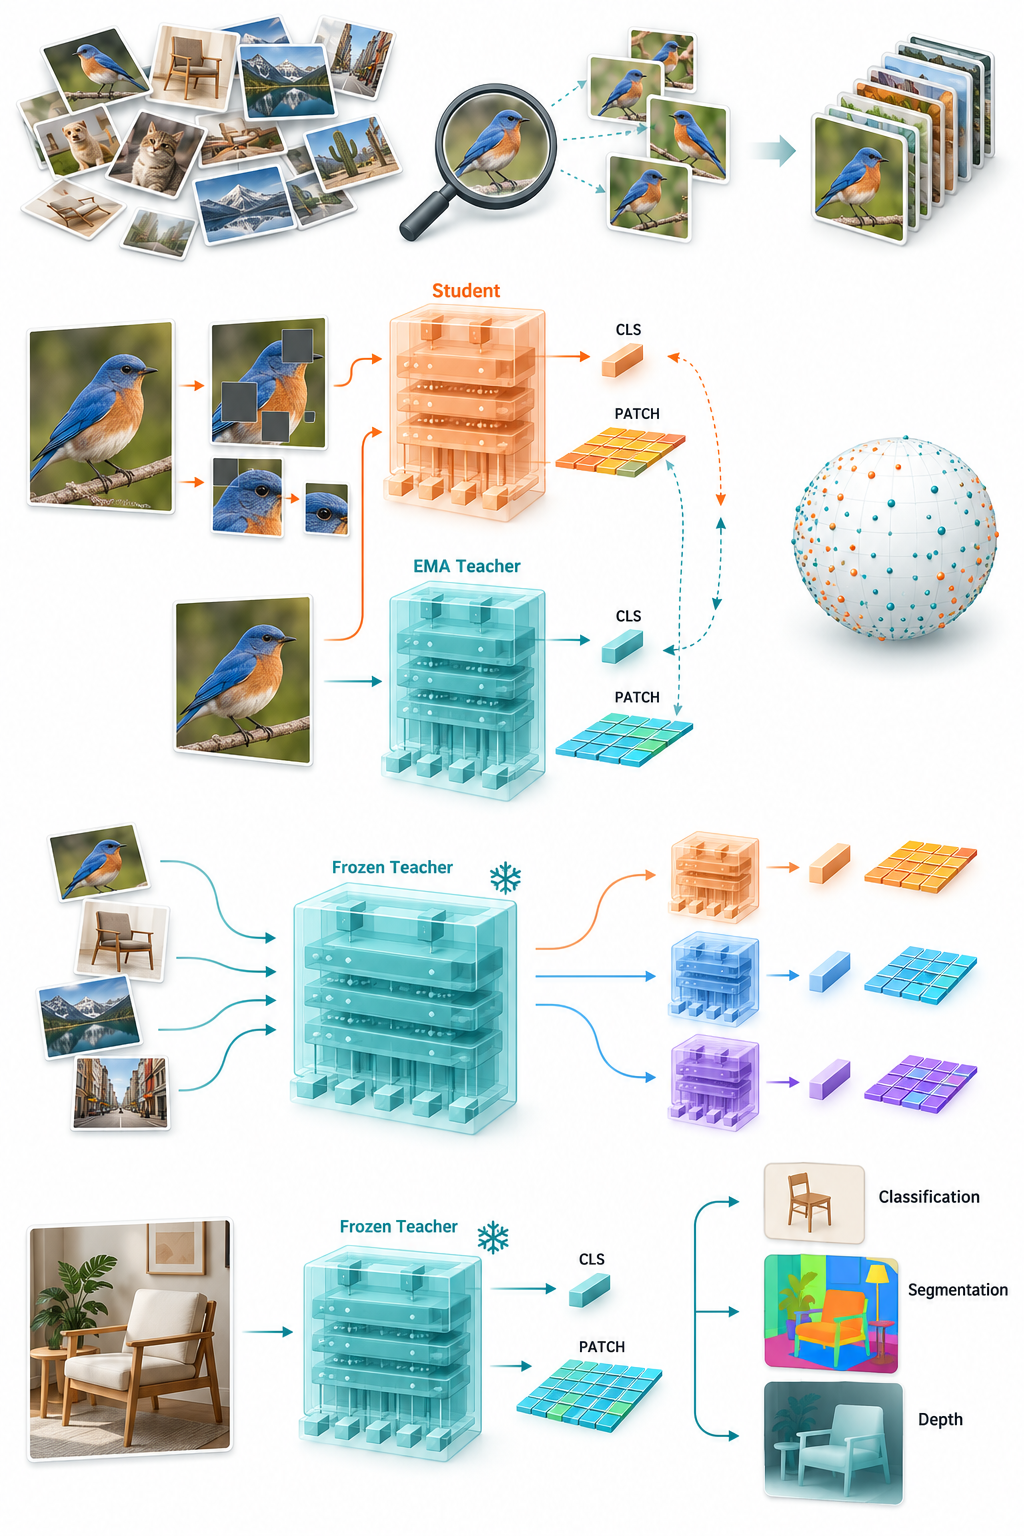
\includegraphics[trim=#1bp \bt bp \rt bp #2bp,clip,width=\aw]{dinov2-imagegen-draft.png}};
\endgroup}
\begin{document}
\begin{tikzpicture}[x=.3mm,y=-.3mm]
\path[use as bounding box](0,0)rectangle(720,2090);
\fill[white](0,0)rectangle(720,2090);
\headat{360}{33}{705}{DINOv2：从图像中学出可复用的特征}
\textat{360}{75}{700}{筛数据 → 自监督预训练 → 蒸馏 → 冻结骨干做任务}

% A: data curation.
\draw[box,fill=tealbg](8,108)rectangle(712,370);
\headat{360}{137}{680}{A\quad 用图像相似度筛数据}
\art{12}{0}{385}{258}{25}{171}{190}
\art{400}{70}{160}{180}{280}{168}{115}
\art{806}{33}{214}{220}{532}{168}{130}
\draw[ar](218,235)--(270,235);
\draw[ar](400,235)--(506,235);
\smallat{116}{319}{205}{原始图池 + 种子图集}
\smallat{350}{319}{265}{去重 → 特征检索 → 再平衡}
\textat{597}{326}{194}{LVD-142M}
\smallat{360}{353}{680}{用图像检索图像；预训练目标不用类别标签或描述文字}

% B: two input routes with unshared CLS and patch heads.
\draw[box,draw=warm!55,fill=warmbg](8,385)rectangle(712,1062);
\headat{360}{416}{680}{B\quad 全局一致 + 被遮挡的局部一致}
\smallat{360}{452}{675}{同一张图的多视图；学生学预测，教师提供目标分布}
\textat{107}{491}{180}{学生输入}
\textat{287}{491}{190}{学生网络}
\textat{476}{491}{190}{两个独立头}
\art{207}{314}{125}{140}{39}{524}{110}
\art{207}{456}{76}{80}{40}{681}{43}
\smallat{105}{665}{178}{遮挡全局图}
\smallat{129}{709}{82}{局部图}
\art{383}{307}{164}{214}{225}{523}{128}
\draw[ar](164,588)--(216,588);
\draw[ar](170,705)--(204,705)--(204,613)--(216,613);
\draw[box,draw=warm](396,529)rectangle(555,583);
\textat{475}{557}{151}{CLS → DINO 头}
\draw[box,draw=warm](396,611)rectangle(555,666);
\textat{475}{639}{152}{patch → iBOT 头}
\draw[ar](358,579)--(376,579)--(376,556)--(391,556);
\draw[ar](358,608)--(376,608)--(376,639)--(391,639);
\smallat{633}{580}{125}{学生 softmax\\教师 SK\\3 轮归一化}
\smallat{289}{723}{190}{梯度更新学生参数}

\textat{106}{756}{185}{教师输入}
\textat{287}{756}{205}{EMA 教师}
\art{175}{598}{139}{169}{50}{790}{105}
\smallat{105}{941}{183}{未遮挡全局图}
\art{383}{585}{166}{216}{225}{786}{128}
\draw[ar](161,858)--(216,858);
\draw[box](396,791)rectangle(555,845);
\textat{475}{818}{151}{CLS → DINO 头}
\draw[box](396,873)rectangle(555,927);
\textat{475}{900}{152}{patch → iBOT 头}
\draw[ar](358,840)--(376,840)--(376,818)--(391,818);
\draw[ar](358,874)--(376,874)--(376,900)--(391,900);
% target comparisons on the right, with separate routes.
\draw[sup](559,818)--(584,818)--(584,557)--(559,557);
\draw[sup](559,900)--(684,900)--(684,639)--(559,639);
\smallat{625}{719}{115}{DINO\\跨视图\\CLS 对齐}
\smallat{632}{856}{125}{iBOT\\同位置\\遮挡 patch}
% EMA only affects teacher, no backpropagation path to teacher.
\draw[sup](212,654)--(192,654)--(192,972)--(287,972)--(287,954);
\smallat{307}{1008}{360}{$\theta_t\leftarrow m\theta_t+(1-m)\theta_s$\\教师随学生做指数滑动平均}
\art{792}{435}{220}{238}{514}{984}{60}
\smallat{646}{1007}{125}{KoLeo\\归一化 CLS\\拉开近邻距离}

% C: fixed large teacher and final student EMA, explicitly not stage B EMA teacher.
\draw[box,draw=warm!55,fill=warmbg](8,1077)rectangle(712,1443);
\headat{360}{1110}{680}{C\quad 把大模型的特征蒸馏给小模型}
\art{285}{893}{244}{246}{47}{1151}{169}
\art{670}{832}{90}{95}{400}{1170}{72}
\art{670}{934}{90}{96}{491}{1170}{72}
\art{670}{1038}{90}{99}{582}{1170}{72}
\textat{135}{1351}{245}{冻结 ViT-g 教师\\1.1B 参数}
\textat{527}{1285}{290}{ViT-S / B / L 学生}
\draw[sup](226,1225)--(379,1225);
\smallat{306}{1186}{166}{固定目标}
\smallat{307}{1264}{180}{DINO + iBOT}
\smallat{531}{1337}{330}{学生继续训练；另存学生 EMA\\最终使用学生的 EMA 模型}
\textat{360}{1410}{670}{去掉遮挡与 stochastic depth；iBOT 作用两个全局视图}

% D: frozen feature extraction and task-specific trained heads.
\draw[box,draw=blue!55,fill=bluebg](8,1458)rectangle(712,2052);
\headat{360}{1491}{680}{D\quad 冻结骨干，任务头读取图像信息}
\art{26}{1225}{209}{238}{32}{1531}{132}
\art{301}{1254}{185}{211}{237}{1531}{132}
\draw[ar](169,1611)--(226,1611);
\smallat{100}{1710}{171}{输入图像}
\textat{304}{1710}{215}{冻结编码器}
\draw[box,draw=blue](441,1538)rectangle(686,1602);
\textat{565}{1570}{237}{全局 CLS 特征 $z$}
\draw[box,draw=blue](441,1631)rectangle(686,1696);
\textat{565}{1663}{237}{局部 patch 特征 $f_i$}
\draw[ar](374,1593)--(412,1593)--(412,1570)--(436,1570);
\draw[ar](374,1629)--(412,1629)--(412,1663)--(436,1663);
\smallat{360}{1913}{665}{$224\times224$ 图、$14\times14$ patch → $16\times16=256$ 个 patch\\ViT-g 的每个 token 为 $1536$ 维}
\draw[ar](565,1605)--(701,1605)--(701,1734)--(141,1734)--(141,1810);
\draw[ar,preaction={draw=bluebg,line width=5pt}](565,1699)--(565,1720)--(360,1720)--(360,1810);

\draw[ar](565,1720)--(690,1720)--(690,1803)--(579,1803)--(579,1810);
\draw[box,draw=blue](44,1815)rectangle(238,1882);
\textat{141}{1849}{182}{分类 / 图像检索}
\draw[box,draw=blue](263,1815)rectangle(457,1882);
\textat{360}{1849}{182}{语义分割}
\draw[box,draw=blue](482,1815)rectangle(676,1882);
\textat{579}{1849}{182}{单目深度}
\smallat{360}{1973}{665}{下游分类 / 分割 / 深度头用任务标注训练；骨干保持冻结\\深度线性读出会拼接 CLS；检索可直接比较特征相似度}
\smallat{360}{2030}{665}{暖色：训练 / 目标更新\qquad 蓝色：冻结特征的下游用法}
\smallat{360}{2076}{700}{实线：前向数据流\qquad 虚线：目标或 EMA 更新\qquad 区域 A–D 对应正文}
\end{tikzpicture}
\end{document}
